\newpage
\section{}

\subsection{Pure water was quasi-statically cooled from room temperature to $-5^{\circ}$C under $1$ atm pressure. Calculate the critical nucleus radius under these conditions. Assume the nucleus is spherical, the latent heat is $6$ kJ/mol, the interfacial energy between ice and water is $30$ mJ/m$^2$, and the density of ice is $1$ g/cm$^3$.}

The critical nucleus radius can be calculated using the following equation: 
\begin{align}
  \label{eq:r01}
  r^*&=\dfrac{-2\gamma}{\Delta G_v},
\end{align}
where $\gamma$ is the surface free energy, and $\Delta G_v$ is the volume free energy change. Because $\Delta G_v$ is a function of temperature:
\begin{align}
  \label{eq:deltagv}
  \Delta G_v&= \dfrac{\Delta H_f\left(T_m-T\right)}{T_m}.
\end{align}
Substituting equation \ref{eq:deltagv} in \ref{eq:r01} gives: 
\begin{align}
  \label{eq:nucleus_radius}
  r^*&=\left(\dfrac{-2\gamma T_m}{\Delta H_f}\right)\left(\dfrac{1}{T_m - T}\right),
\end{align}
where $\gamma$ is the surface free energy in J/m$^2$, $\Delta H_f$ is the the latent heat of fusion in J/m$^3$, $T_m$ is the melting temperature in K and $T$ is the transformation temperature in K \citep[p.~346-347]{callister2010materials}.

Because the latent heat provided in the problem is given in kJ/mol, it is necessary to convert to J/m$^3$ for the calculation. Using the density of ice and the molar mass for water, 18.01528 g/mol:
\begin{align}
  \begin{split}
    \left(\dfrac{6000\text{ J}}{\text{mol}}\right)\left(\dfrac{1\text{ mol}}{18.01528\text{ g}}\right)\left(\dfrac{1\text{ g}}{\text{cm}^3}\right)\left(\dfrac{100\text{ cm}}{1\text{ m}}\right)^3&=333050610.370752 \text{ J/m}^3 \\
  &\approx 3.33\times10^{-8} \text{ J/m}^3
  \end{split}
  \label{eq:deltaH_calculation}
\end{align}

Using equation \ref{eq:nucleus_radius}, the critical nucleus radius can be calculated:
\begin{align}
  \label{eq:radius}
  \begin{split}
    r^*&=\left(\dfrac{-2*0.03*273}{-333050610.370752}\right)\left(\dfrac{1}{273-268}\right)=9.836342879999998\times 10^{-9}\text{ m} \\ 
    r^*&\approx 9.84\times 10^{-9} \text{ m}
  \end{split}
\end{align}

\begin{mdframed}
The critical nucleus radius for water quasi-statically cooled from room temperature to $-5^{\circ}$ is 9.84 nm.
\end{mdframed}

\subsection{Explain how the critical nucleus radius changes if the pure water is
further cooled, including the reason.}

To visualize the changes of the radius with further cooling water, the critical radius was calculated for different cooling temperatures, with a range of cooling temperatures of $-5$ to $-270^{\circ}$C (near absolute zero temperature), using equation \ref{eq:nucleus_radius}. The results were plotted in a graph, which is shown in figure \ref{fig:critical_radius}:

\begin{figure}[h]
    \centering
    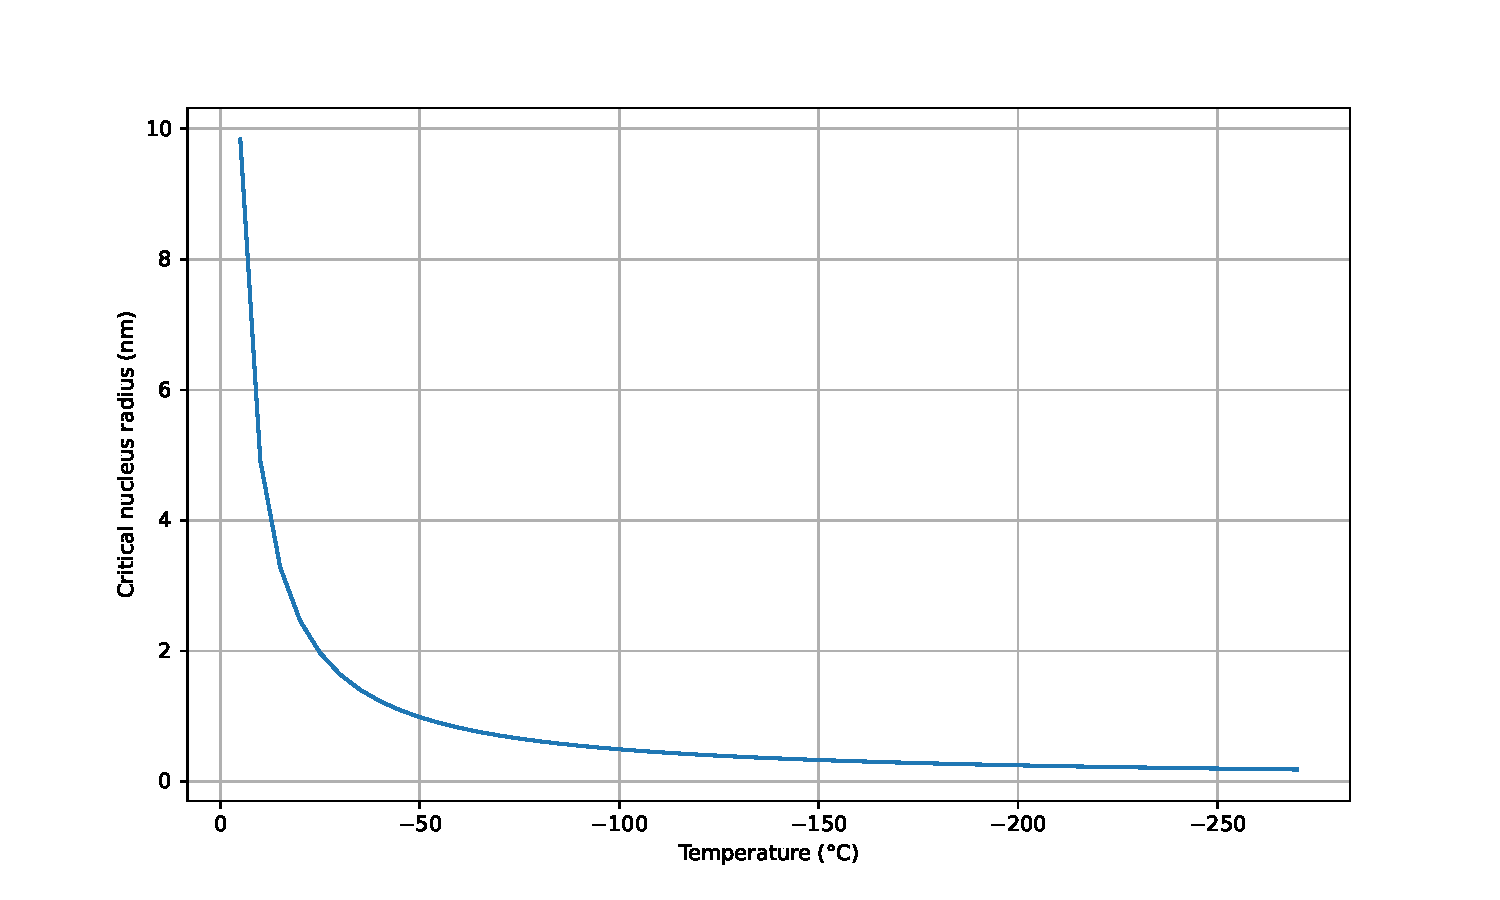
\includegraphics[width=1\textwidth]{graficas/critical_radius.pdf}
    \caption{Critical nucleus radius as a function of temperature for water cooled in a range of temperature from $-5$ to $-270^{\circ}$ C. \\
    \textit{Source: Visualization by the author (code available at \citet{mygit})}}
    \label{fig:critical_radius}
\end{figure}

Figure \ref{fig:critical_radius} shows the nucleus radius as a function of temperature, it can be seen that as the critical nucleus radius descends as does the temperature. This behavior is expected from equation \ref{eq:nucleus_radius}, where the critical radius is proportionally inverse to the temperature difference of the cooling temperature and the melting temperature. As the cooling temperature is lower, the difference between the the melting temperature and the cooling temperature increases, and the critical radius becomes smaller.
The decrease in the critical radius continues reaching a nearly asymptotic behavior that starts around $-200^{\circ}$ C  temperature, with an approximate value for the radius of $0.2$ nm, as it gets closer to the absolute temperature. 

%\shnote{me falta explicar por que el radio cambia de esta manera, segun yo como en la ecuacion es inverso al delta t entonces deberia de disminuir el radio conforme el delta t se hace mas grande, es decir al enfriar hasta temperaturas mas bajas}